% Spectral namer (app/spectral_match/namer/model.py) - publication schematic. Build:
%   C:/Users/FITT/tools/tectonic/tectonic.exe namer_network.tex
\documentclass[tikz,border=6pt]{standalone}
\usepackage[T1]{fontenc}
\usepackage{lmodern}
\usepackage{amsmath,amssymb,bm}
\usetikzlibrary{positioning,arrows.meta,calc,fit,backgrounds,shapes.misc,decorations.pathreplacing}
\renewcommand{\familydefault}{\sfdefault}

\definecolor{ink}{HTML}{1F2933}
\definecolor{stem}{HTML}{DCE8F5}\definecolor{stemE}{HTML}{3D6FA8}
\definecolor{pix}{HTML}{FBE6D4}\definecolor{pixE}{HTML}{C0662B}
\definecolor{lib}{HTML}{DFF0E3}\definecolor{libE}{HTML}{3E8E57}
\definecolor{mat}{HTML}{ECE4F5}\definecolor{matE}{HTML}{6D4FA0}
\definecolor{loss}{HTML}{B3261E}\definecolor{ring}{HTML}{B9C3CE}\definecolor{grid}{HTML}{E8ECF0}

\tikzset{
  >={Stealth[length=2.2mm]}, every node/.style={font=\footnotesize, text=ink},
  box/.style={draw, rounded corners=2pt, line width=0.7pt, align=center, inner sep=4pt, minimum height=9mm},
  stembox/.style={box, fill=stem, draw=stemE, minimum width=27mm},
  pixbox/.style={box, fill=pix, draw=pixE},
  libbox/.style={box, fill=lib, draw=libE},
  matbox/.style={box, fill=mat, draw=matE},
  vec/.style={draw=ink!70, fill=white, rounded corners=1pt, inner sep=2.5pt, font=\footnotesize},
  op/.style={circle, draw=ink, fill=white, inner sep=0.6pt, font=\scriptsize, minimum size=4.6mm},
  flow/.style={->, line width=0.7pt, draw=ink!85},
  lossbox/.style={draw=loss, dashed, rounded corners=2pt, text=loss, font=\scriptsize, align=center, inner sep=3pt},
  lossflow/.style={->, dashed, draw=loss, line width=0.6pt},
  dim/.style={font=\scriptsize, text=ink!60},
}

% a small spectrum glyph: \spec{x}{y}{colour}
\newcommand{\spec}[3]{%
  \draw[#3, line width=0.8pt] plot[smooth] coordinates {
    ($(#1,#2)+(-0.55,-0.22)$) ($(#1,#2)+(-0.35,0.05)$) ($(#1,#2)+(-0.15,0.18)$) ($(#1,#2)+(0.0,-0.05)$)
    ($(#1,#2)+(0.15,0.12)$) ($(#1,#2)+(0.35,-0.15)$) ($(#1,#2)+(0.55,0.0)$)};
  \draw[ink!50, line width=0.4pt] ($(#1,#2)+(-0.6,-0.3)$) -- ($(#1,#2)+(0.6,-0.3)$);}

\begin{document}
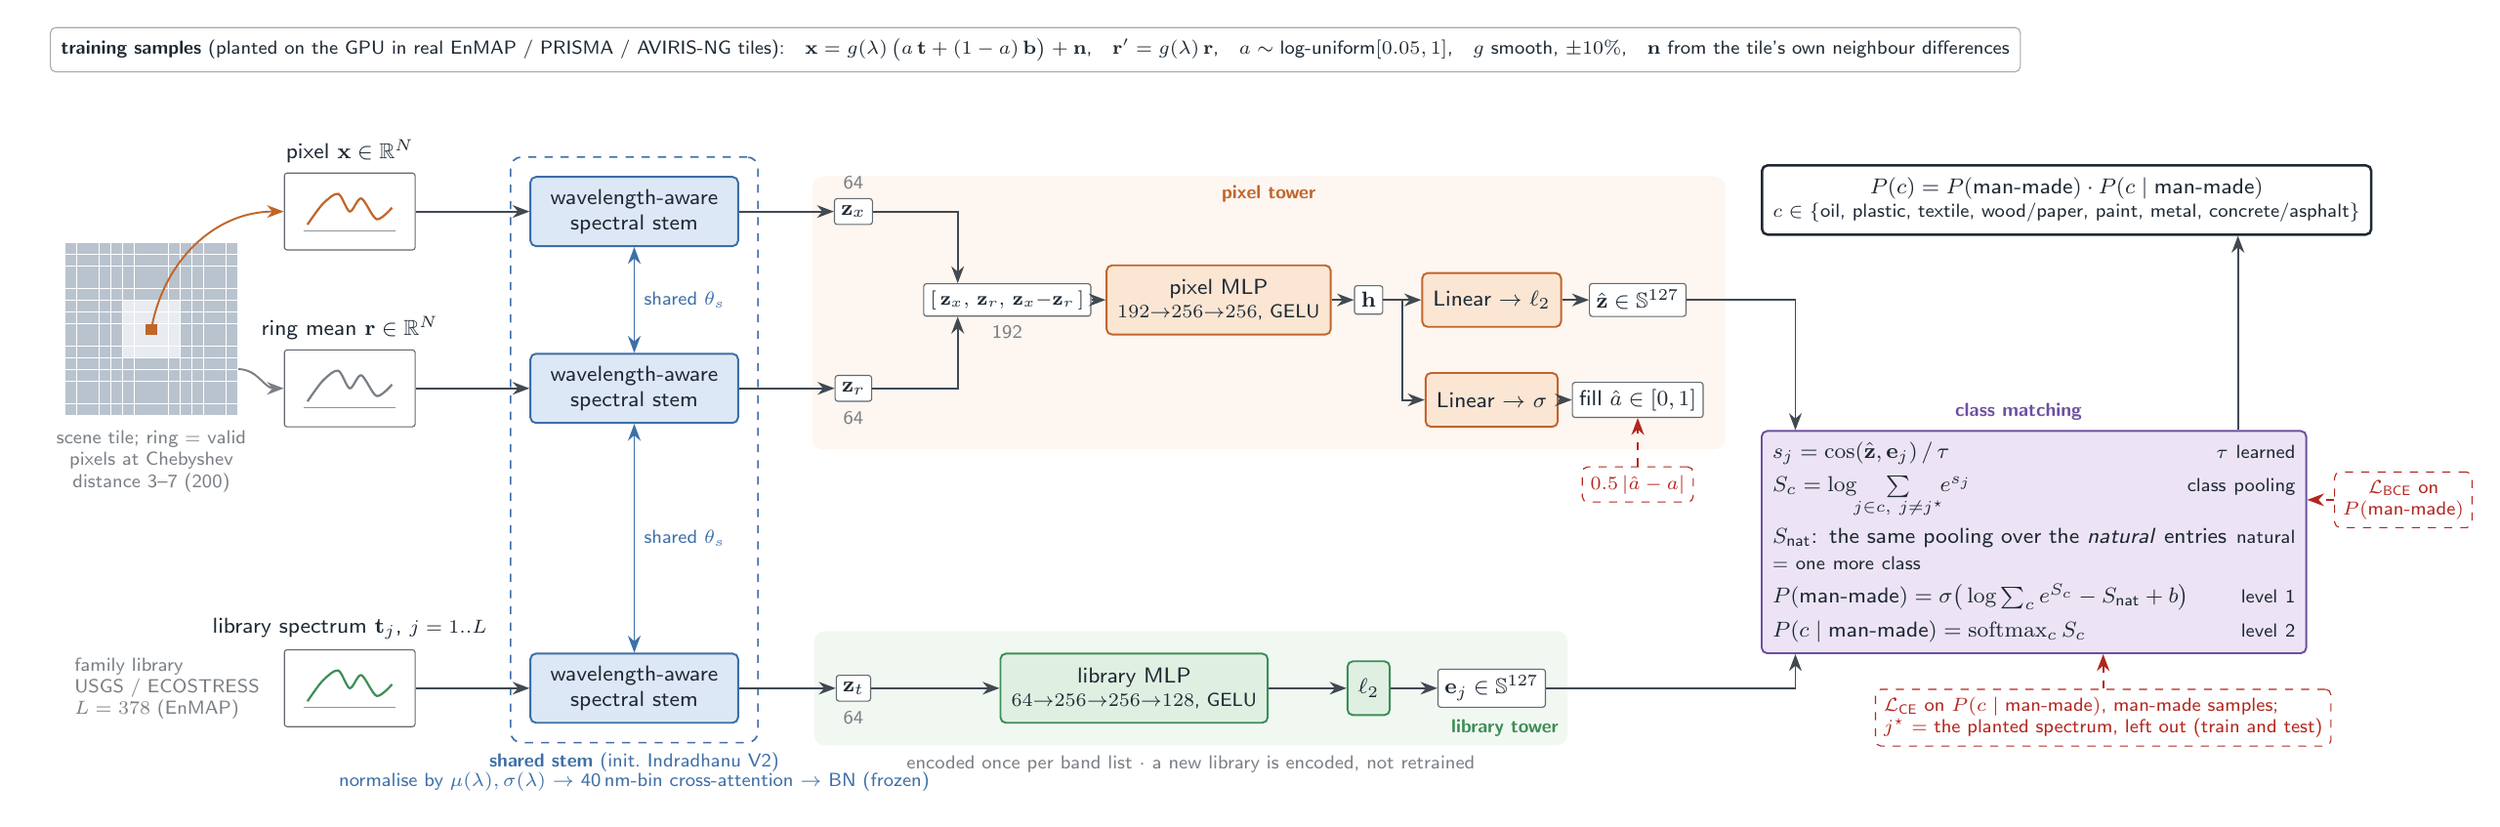
\begin{tikzpicture}

% ---------------- scene patch with the ring ----------------
\begin{scope}[shift={(-4.9,3.55)}]
  \foreach \i in {0,...,14}{\foreach \j in {0,...,14}{
    \pgfmathtruncatemacro{\di}{abs(\i-7)}\pgfmathtruncatemacro{\dj}{abs(\j-7)}
    \pgfmathtruncatemacro{\d}{max(\di,\dj)}
    \ifnum\d>2 \def\c{ring}\else\def\c{grid}\fi
    \ifnum\d=0 \def\c{pixE}\fi
    \fill[\c] (\i*0.15,\j*0.15) rectangle ++(0.14,0.14);}}
  \node[dim, align=center, text width=30mm, anchor=north] at (1.12,-0.08) {scene tile; ring = valid\\pixels at Chebyshev\\distance 3--7 (200)};
  \coordinate (pxc) at (1.12,1.12);
  \coordinate (ringR) at (2.25,0.6);
\end{scope}

% ---------------- inputs ----------------
\node[vec, minimum width=17mm, minimum height=10mm] (x) at (-1.2,6.2) {};
\spec{-1.2}{6.25}{pixE}
\node[above=0pt of x] {pixel $\mathbf{x}\in\mathbb{R}^{N}$};
\node[vec, minimum width=17mm, minimum height=10mm] (r) at (-1.2,3.9) {};
\spec{-1.2}{3.95}{ink!60}
\node[above=0pt of r] {ring mean $\mathbf{r}\in\mathbb{R}^{N}$};
\draw[flow, pixE] (pxc) to[out=80,in=180] (x.west);
\draw[flow, ink!60] (ringR) to[out=0,in=180] (r.west);

\node[vec, minimum width=17mm, minimum height=10mm] (t) at (-1.2,0.0) {};
\spec{-1.2}{0.05}{libE}
\node[above=0pt of t, align=center] {library spectrum $\mathbf{t}_j$, {\scriptsize $j = 1..L$}};
\node[dim, align=left, anchor=east] at (-2.25,0.0) {family library\\USGS / ECOSTRESS\\$L=378$ (EnMAP)};

% ---------------- shared stem ----------------
\node[stembox] (sx) at (2.5,6.2) {wavelength-aware\\spectral stem};
\node[stembox] (sr) at (2.5,3.9) {wavelength-aware\\spectral stem};
\node[stembox] (st) at (2.5,0.0) {wavelength-aware\\spectral stem};
\draw[flow] (x) -- (sx); \draw[flow] (r) -- (sr); \draw[flow] (t) -- (st);
\begin{scope}[on background layer]
  \node[draw=stemE, dashed, rounded corners=4pt, fit=(sx)(sr)(st), inner sep=7pt, line width=0.6pt] (stemgrp) {};
\end{scope}
\draw[<->, stemE, line width=0.6pt] (sx.south) -- (sr.north) node[midway, right, font=\scriptsize, text=stemE] {shared $\theta_s$};
\draw[<->, stemE, line width=0.6pt] (sr.south) -- (st.north) node[midway, right, font=\scriptsize, text=stemE, align=left] {shared $\theta_s$};
\node[font=\scriptsize, text=stemE, align=center, anchor=north] at (stemgrp.south) {\textbf{shared stem} (init.\ Indradhanu V2)\\[-1pt]
  normalise by $\mu(\lambda),\sigma(\lambda)$ $\to$ 40\,nm-bin cross-attention $\to$ BN (frozen)};

% ---------------- pixel tower ----------------
\node[vec] (zx) at (5.35,6.2) {$\mathbf{z}_x$}; \node[dim, above=0pt of zx] {64};
\node[vec] (zr) at (5.35,3.9) {$\mathbf{z}_r$}; \node[dim, below=0pt of zr] {64};
\draw[flow] (sx) -- (zx); \draw[flow] (sr) -- (zr);
\node[vec, align=center, font=\scriptsize] (cat) at (7.35,5.05) {$[\,\mathbf{z}_x,\,\mathbf{z}_r,\,\mathbf{z}_x{-}\mathbf{z}_r\,]$};
\node[dim, below=0pt of cat] {192};
\draw[flow] (zx.east) -| ($(cat.north west)+(0.45,0)$);
\draw[flow] (zr.east) -| ($(cat.south west)+(0.45,0)$);
\node[pixbox] (pmlp) at (10.1,5.05) {pixel MLP\\[-1pt]{\scriptsize $192{\to}256{\to}256$, GELU}};
\draw[flow] (cat) -- (pmlp);
\node[vec] (h) at (12.05,5.05) {$\mathbf{h}$};
\draw[flow] (pmlp) -- (h);

% heads
\node[pixbox, minimum height=7mm] (hz) at (13.65,5.05) {Linear $\to$ $\ell_2$};
\node[pixbox, minimum height=7mm] (hf) at (13.65,3.75) {Linear $\to$ $\sigma$};
\foreach \n in {hz,hf} \draw[flow] (h.east) -- ++(0.25,0) |- (\n.west);
\node[vec] (z) at (15.55,5.05) {$\hat{\mathbf{z}}\in\mathbb{S}^{127}$};
\node[vec] (fill) at (15.55,3.75) {fill $\hat a\in[0,1]$};
\draw[flow] (hz) -- (z); \draw[flow] (hf) -- (fill);
\begin{scope}[on background layer]
  \node[fill=pix!35, rounded corners=4pt, fit=(zx)(zr)(cat)(pmlp)(h)(hz)(hf)(z)(fill), inner sep=8pt] (pixgrp) {};
\end{scope}
\node[font=\scriptsize\bfseries, text=pixE, anchor=north] at (pixgrp.north) {pixel tower};

% ---------------- library tower ----------------
\node[vec] (zt) at (5.35,0.0) {$\mathbf{z}_t$}; \node[dim, below=0pt of zt] {64};
\draw[flow] (st) -- (zt);
\node[libbox] (lmlp) at (9.0,0.0) {library MLP\\[-1pt]{\scriptsize $64{\to}256{\to}256{\to}128$, GELU}};
\draw[flow] (zt) -- (lmlp);
\node[libbox, minimum height=7mm] (ln) at (12.05,0.0) {$\ell_2$};
\draw[flow] (lmlp) -- (ln);
\node[vec] (e) at (13.65,0.0) {$\mathbf{e}_j\in\mathbb{S}^{127}$};
\draw[flow] (ln) -- (e);
\begin{scope}[on background layer]
  \node[fill=lib!45, rounded corners=4pt, fit=(zt)(lmlp)(ln)(e), inner sep=8pt] (libgrp) {};
\end{scope}
\node[font=\scriptsize\bfseries, text=libE, anchor=south east] at (libgrp.south east) {library tower};
\node[dim, align=center, anchor=north] at (libgrp.south) {encoded once per band list $\cdot$ a new library is encoded, not retrained};

% ---------------- matching ----------------
\node[matbox, align=left, text width=68mm, anchor=west] (match) at (17.15,1.9) {%
  $s_j = \cos(\hat{\mathbf{z}},\mathbf{e}_j)\,/\,\tau$ \hfill {\scriptsize $\tau$ learned}\\[3pt]
  $S_c = \log\!\!\sum\limits_{j\in c,\ j\neq j^{\star}}\!\! e^{s_j}$ \hfill {\scriptsize class pooling}\\[3pt]
  $S_{\text{nat}}$: the same pooling over the \emph{natural} entries \hfill {\scriptsize natural = one more class}\\[3pt]
  $P(\text{man-made}) = \sigma\big(\log\sum_{c} e^{S_c} - S_{\text{nat}} + b\big)$ \hfill {\scriptsize level 1}\\[3pt]
  $P(c\mid\text{man-made}) = \operatorname{softmax}_c S_c$ \hfill {\scriptsize level 2}};
\node[font=\scriptsize\bfseries, text=matE, anchor=south] at ($(match.north)+(-0.2,0)$) {class matching};
\draw[flow] (z.east) -| ($(match.north west)+(0.45,0)$);
\draw[flow] (e.east) -| ($(match.south west)+(0.45,0)$);

\node[box, fill=white, draw=ink, line width=0.9pt, align=center, anchor=west] (out) at (17.15,6.35) {%
  $P(c) = P(\text{man-made})\cdot P(c\mid\text{man-made})$\\[-1pt]
  {\scriptsize $c\in\{$oil, plastic, textile, wood/paper, paint, metal, concrete/asphalt$\}$}};
\coordinate (mtop) at ($(match.north east)+(-0.9,0)$);
\draw[flow] (mtop) -- (mtop |- out.south);

% ---------------- losses ----------------
\node[lossbox, anchor=west] (lbce) at ($(match.east)+(0.35,0.55)$) {$\mathcal{L}_{\text{BCE}}$ on\\$P(\text{man-made})$};
\draw[lossflow] (lbce.west) -- (lbce.west -| match.east);
\node[lossbox] (lfill) at (15.55,2.65) {$0.5\,\lvert \hat a - a\rvert$};
\draw[lossflow] (lfill.north) -- (fill.south);
\node[lossbox, align=left, anchor=north] (lce) at ($(match.south)+(0.9,-0.45)$) {$\mathcal{L}_{\text{CE}}$ on $P(c\mid\text{man-made})$, man-made samples;\\
  $j^{\star}$ = the planted spectrum, left out (train and test)};
\draw[lossflow] (lce.north) -- (lce.north |- match.south);

% ---------------- training input note ----------------
\node[draw=ink!40, rounded corners=2pt, align=left, font=\scriptsize, inner sep=4pt, anchor=north west] at (-5.1,8.6) {%
  \textbf{training samples} (planted on the GPU in real EnMAP / PRISMA / AVIRIS-NG tiles):\quad
  $\mathbf{x} = g(\lambda)\,\big(a\,\mathbf{t} + (1-a)\,\mathbf{b}\big) + \mathbf{n}$,\quad $\mathbf{r}' = g(\lambda)\,\mathbf{r}$,\quad
  $a \sim \text{log-uniform}[0.05,1]$,\quad $g$ smooth, $\pm10\%$,\quad $\mathbf{n}$ from the tile's own neighbour differences};

\end{tikzpicture}
\end{document}
